%!TEX root = ../rapport.tex

\section{Déploiement}

Nous allons voir ici comment générer et déployer l'exécutable .apk sur la Set-Top Box ainsi que le fichier .war pour le serveur.

\subsection{Set-Top Box}
La STB est connectée au réseau local et possède une adresse IP. L'utilitaire \textbf{adb} permet de se connecter sur la STB.
\begin{lstlisting}[caption={Connection à la Set-Top Box via ADB}]
adb connect IP_ADDR
\end{lstlisting}

A présent, la box est connectée comme n'importe quel terminal Android. Il est donc possible, via Eclipse, d'afficher les logs du terminal, ainsi que de compiler et déployer le programme.

\medskip

Sauf que le déploiement ne \textbf{fonctionne pas}. En effet, sans doutes à cause d'options de compilation rajoutées par Eclipse, l'application n'est pas déployée correctement et n'est pas reconnue par la box. Ce qu'il faut donc faire, c'est construire le fichier .apk avec Eclipse, puis l'envoyer manuellement sur la box via l'utilitaire adb.

\medskip

L'application est générée dans le chemin suivant:

\textit{APP\_DIRECTORY/bin/app\_name.apk}

\medskip

Il suffit alors d'utiliser adb.

\begin{lstlisting}[caption={Envoi du fichier apk sur la Set-Top Box}]
adb push APP_DIRECTORY/bin/app_name.apk /system/data
\end{lstlisting}

Le répertoire \textbf{/system/data} n'est accessible qu'en tant qu'utilisateur root.

\medskip

L'application est à présent déployée sur notre STB.
\subsection{Serveur}

Le dossier \textbf{webapp} du répertoire d'installation de Jetty est le dossier de déploiement du serveur. Lorsqu'un fichier est déposé dans ce répertoire, il est automatiquement lu et déployé par Jetty s'il est démarré, ou le fera lorsqu'il sera lancé.

\medskip

La compilation de la partie serveur se fait avec Maven comme déjà expliqué. En se mettant dans le répertoire racine de l'application, caractérisé par le dossier \textbf{pom.xml} que Maven va lire, il suffit de lancer la commande 
\begin{lstlisting}[caption=Commande Maven pour construire le fichier déployable]
mvn clean install
\end{lstlisting}

On remarque qu'à la première exécution de cette commande, un dossier \textbf{target} est créé.

\begin{figure}[H]
    \begin{center}
        \centering 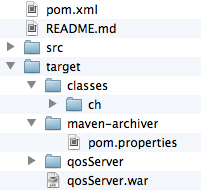
\includegraphics[width=120px]{00_media/target_arb}
        \caption{Target contenu}
    \end{center}
\end{figure}

\begin{itemize}
	\item classes: répertoire contenant les classes compilées de l'application
	\item maven-archiver: contient le fichier pom.properties. Ce sont les propriétés tirées du fichier pom.xml
	\item qosServer: dossier contenant l'extraction du fichier war. Il s'agit du projet déployé
	\item qosServer.war: fichier conteneur permettant le déploiement de l'application sur le serveur
\end{itemize}

\medskip

Il suffit de copier le fichier .war dans le dossier webapp de Jetty pour pouvoir le déployer.

\begin{lstlisting}[caption=Copie du fichier war vers Jetty]
	cp SERVER_DIRECTORY/target/app_name.war JETTY_DIRECTORY/webapp
\end{lstlisting}

L'application est déployée à l'adresse:

\textit{protocole://server\_name:portNumber/war\_file\_name}